
%% bare_conf_compsoc.tex
%% V1.4b
%% 2015/08/26
%% by Michael Shell
%% See:
%% http://www.michaelshell.org/
%% for current contact information.
%%
%% This is a skeleton file demonstrating the use of IEEEtran.cls
%% (requires IEEEtran.cls version 1.8b or later) with an IEEE Computer
%% Society conference paper.
%%
%% Support sites:
%% http://www.michaelshell.org/tex/ieeetran/
%% http://www.ctan.org/pkg/ieeetran
%% and
%% http://www.ieee.org/

%%*************************************************************************
%% Legal Notice:
%% This code is offered as-is without any warranty either expressed or
%% implied; without even the implied warranty of MERCHANTABILITY or
%% FITNESS FOR A PARTICULAR PURPOSE! 
%% User assumes all risk.
%% In no event shall the IEEE or any contributor to this code be liable for
%% any damages or losses, including, but not limited to, incidental,
%% consequential, or any other damages, resulting from the use or misuse
%% of any information contained here.
%%
%% All comments are the opinions of their respective authors and are not
%% necessarily endorsed by the IEEE.
%%
%% This work is distributed under the LaTeX Project Public License (LPPL)
%% ( http://www.latex-project.org/ ) version 1.3, and may be freely used,
%% distributed and modified. A copy of the LPPL, version 1.3, is included
%% in the base LaTeX documentation of all distributions of LaTeX released
%% 2003/12/01 or later.
%% Retain all contribution notices and credits.
%% ** Modified files should be clearly indicated as such, including  **
%% ** renaming them and changing author support contact information. **
%%*************************************************************************


\documentclass[conference,compsoc,12pt]{IEEEtran}
%\documentclass[peerreview,12pt]{IEEEtran}

% *** CITATION PACKAGES ***
\usepackage[nocompress]{cite}

% *** GRAPHICS RELATED PACKAGES ***
%
\usepackage[pdftex]{graphicx}
% declare the path(s) where your graphic files are
%\graphicspath{{../images/}}
% and their extensions so you won't have to specify these with
% every instance of \includegraphics
%\DeclareGraphicsExtensions{.jpeg,.png}

% *** MATH PACKAGES ***
\usepackage{amsmath}
% Note that the amsmath package sets \interdisplaylinepenalty to 10000
% thus preventing page breaks from occurring within multiline equations. Use:
%\interdisplaylinepenalty=2500

% *** ALIGNMENT PACKAGES ***
\usepackage{array}

% *** SUBFIGURE PACKAGES ***
\usepackage[caption=false,font=footnotesize,labelfont=sf,textfont=sf]{subfig}

% *** FLOAT PACKAGES ***
%\usepackage{fixltx2e}
%\usepackage{stfloats}
% \usepackage{dblfloatfix}

% *** PDF, URL AND HYPERLINK PACKAGES ***
\usepackage{url}
\usepackage{bm}
%\usepackage{algorithm}
%\usepackage{algorithmic}

% *** Temporary packages ***
\usepackage{lipsum}
\usepackage{pifont}
\usepackage{mdframed}
\usepackage{float}

% Set figures and tables within text for peer-review
\makeatletter
\@ifclasswith{IEEEtran}{peerreview}{\floatplacement{figure}{H}}{\floatplacement{table}{H}}	
\makeatother

%\usepackage{xcolor}
%\newcommand\mytodo[1]{\textcolor{red}{#1}}

% correct bad hyphenation here
\hyphenation{op-tical net-works semi-conduc-tor}

\mdfsetup{%
	skipabove=0.5cm,
	innertopmargin=0.5cm,
	innerbottommargin=0.5cm
}

\begin{document}

% paper title
\title{Feature selection methods for machine learning based docking prediction of Indonesian medicinal plant compounds and HIV-1 protease}


% author names and affiliations
% use a multiple column layout for up to three different
% affiliations
%\author{
%	\IEEEauthorblockN{Rahman Pujianto}
%	\IEEEauthorblockA{Faculty of Computer Science\\
%	Universitas Indonesia\\
%	Email: rahman.pujianto@ui.ac.id\\}
%	\and
%	\IEEEauthorblockN{Heru Suhartanto}
%	\IEEEauthorblockA{Faculty of Computer Science\\
%	Universitas Indonesia\\
%	Email: heru@cs.ui.ac.id\\}
%}

\author{
	\IEEEauthorblockN{
		Rahman Pujianto\IEEEauthorrefmark{1},
		Yohanes Gultom\IEEEauthorrefmark{2}, 
		Ari Wibisono\IEEEauthorrefmark{3},		
		Heru Suhartanto\IEEEauthorrefmark{4}
	}
	\IEEEauthorblockA{
		Faculty of Computer Science,
		Universitas Indonesia\\
		Email: 
		\IEEEauthorrefmark{1}rahman.pujianto@ui.ac.id,
		\IEEEauthorrefmark{2}yohanes.gultom@ui.ac.id,
		\IEEEauthorrefmark{3}ari.w@cs.ui.ac.id 
		\IEEEauthorrefmark{4}heru@cs.ui.ac.id		
	}
}

% make the title area
\maketitle

% As a general rule, do not put math, special symbols or citations
% in the abstract
\begin{abstract}

This research evaluates feature selection methods to reduce number of features required to predict docking result between Indonesian medicinal plant compounds and HIV protease.  

Two feature selection methods on public dataset from PubChem Bioassay and DUD-E decoy which originally have 667 features of molecular description. linear SVM docking predicti of 368 Indonesian herbal chemical compounds with HIV-1 protease from PDB (3OCX). The dataset, which consists 357 positive and 11 negative samples, was labeled by performing manual docking using Autodock. 

This research utilizes machine learning approach to analyze 1,412 chemical compound structures from Indonesian herbal database. From the data, 667 features are extracted from each compounds to build an unlabeled dataset. In order to build a HIV-1 protease inhibitor classification dataset, top 10 of protease inhibitors from related research are used as reference to give positive labels to the unlabeled dataset. Consequently, the remaining 1,402 compounds are labeled as negative. An SVM classifier, which is trained using different public dataset, achieves 66.7\% classification accuracy on it.

\end{abstract}

\IEEEpeerreviewmaketitle

\section{Introduction}

Simulasi dinamika molekular membutuhkan sumber daya komputasi dan waktu yang tidak sedikit. Machine learning harusnya dapat membantu memprediksi hasil simulasi dinamika molekular dengan lebih efisien. Riset ini mencoba melatih model machine learning untuk memprediksi hasil docking dari 368 senyawa herbal indonesia dengan protein HIV-1. \cite{yanuar2014virtual}

\section{Related Work}

TODO


\section{Experiments} \label{Experiments}

Dataset dibuat dengan mencoba melakukan simulasi docking 368 senyawa herbal indonesia dengan protein HIV-1 menggunakan PyRx \& Autodock. Senyawa yang berhasil docking diberi label positif (357 senyawa) dan yang gagal diberi label negatif (11 senyawa).

Eksperimen yang dilakukan:
1. Data latih dan data uji PubChem
2. Data latih PubChem, data uji HerbalDB
3. Data latih dan data uji HerbalDB

Model yang digunakan untuk tiap eksperimen adalah
1. SVM
2. SVM + RFE
3. SVM + WM (GA)
4. (ditambah sesuai kebutuhan)

\begin{figure}
	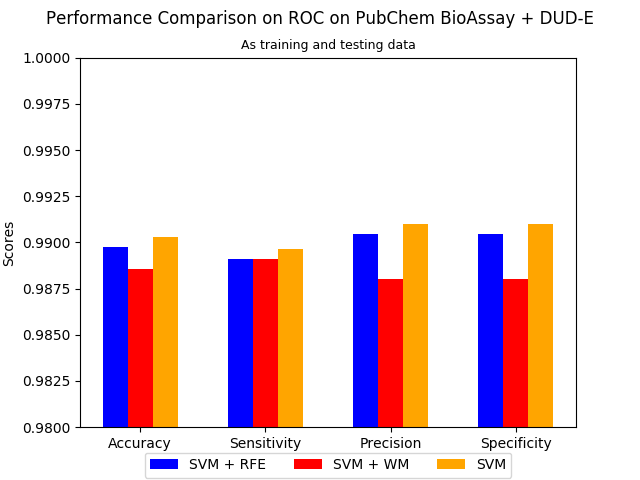
\includegraphics[scale=0.5]{../images/03-evaluate-1_scores_chart.png}
	\caption{Classification performance comparison on PubChem BioAssay + DUD-E dataset}
	\label{fig_performance_comparison_pubchem}
\end{figure}

\begin{figure}
	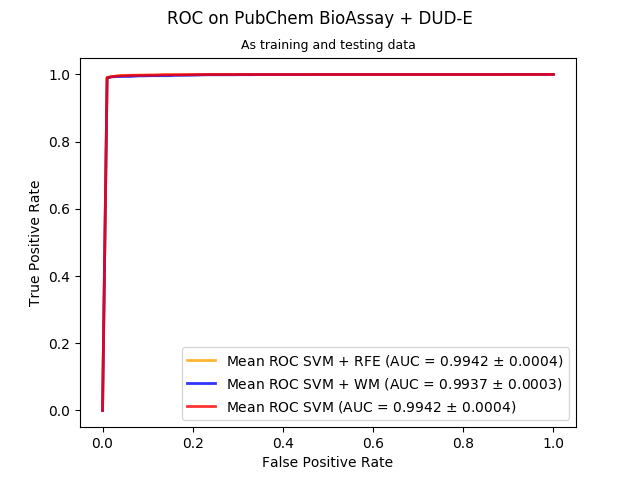
\includegraphics[scale=0.5]{../images/03-evaluate-1_roc_chart.png}
	\caption{AUC ROC comparison on PubChem BioAssay + DUD-E dataset}
	\label{fig_roc_comparison_pubchem}
\end{figure}


\begin{figure}
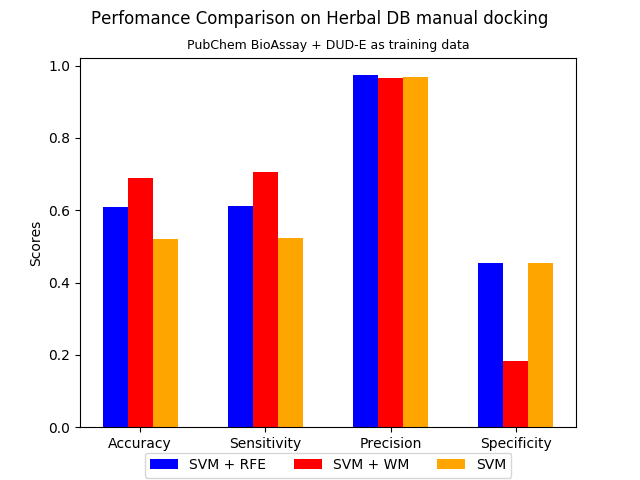
\includegraphics[scale=0.5]{../images/03-evaluate-3_scores_chart.png}
\caption{Classification performance comparison on Herbal DB dataset}
\label{fig_performance_comparison_herbaldb}
\end{figure}

\begin{figure}
	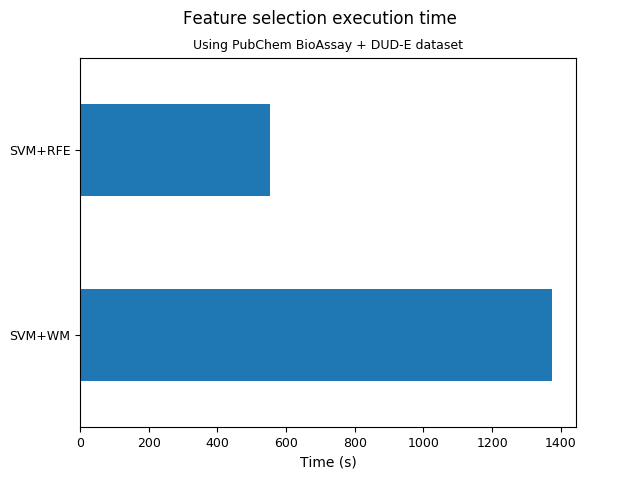
\includegraphics[scale=0.5]{../images/feature_selection_time_comparison.png}
	\caption{Feature selection time comparison}
	\label{fig_feature_selection_time_comparison}
\end{figure}

\begin{figure}
	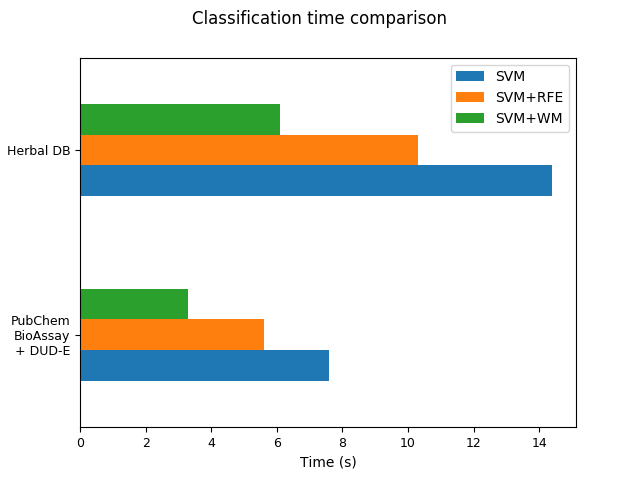
\includegraphics[scale=0.5]{../images/classification_time_comparison.png}
	\caption{Classification time comparison}
	\label{fig_classification_time_comparison}
\end{figure}

\section{Analysis}

Model mana yang paling akurat memprediksi hasil docking senyawa dengan HIV-1

\section{Conclusion}

TODO

% conference papers do not normally have an appendix

% use section* for acknowledgment
%\ifCLASSOPTIONcompsoc
  % The Computer Society usually uses the plural form
%  \section*{Acknowledgments}
%\else
  % regular IEEE prefers the singular form
%  \section*{Acknowledgment}
%\fi

\bibliographystyle{IEEEtran}
\bibliography{../references}

% that's all folks
\end{document}
